\documentclass[tikz,border=15pt]{standalone}
\usepackage[utf8]{inputenc}
\usepackage{tikz}
\usetikzlibrary{shapes,arrows.meta,positioning,calc}

\definecolor{ScoutGreen}{HTML}{005432}
\definecolor{ScoutNavy}{HTML}{002855}
\definecolor{ScoutBlue}{HTML}{006EB6}
\definecolor{ScoutRed}{HTML}{A31920}
\definecolor{ScoutAmber}{HTML}{D97706}
\definecolor{BorderGray}{HTML}{CBD5E1}

\begin{document}
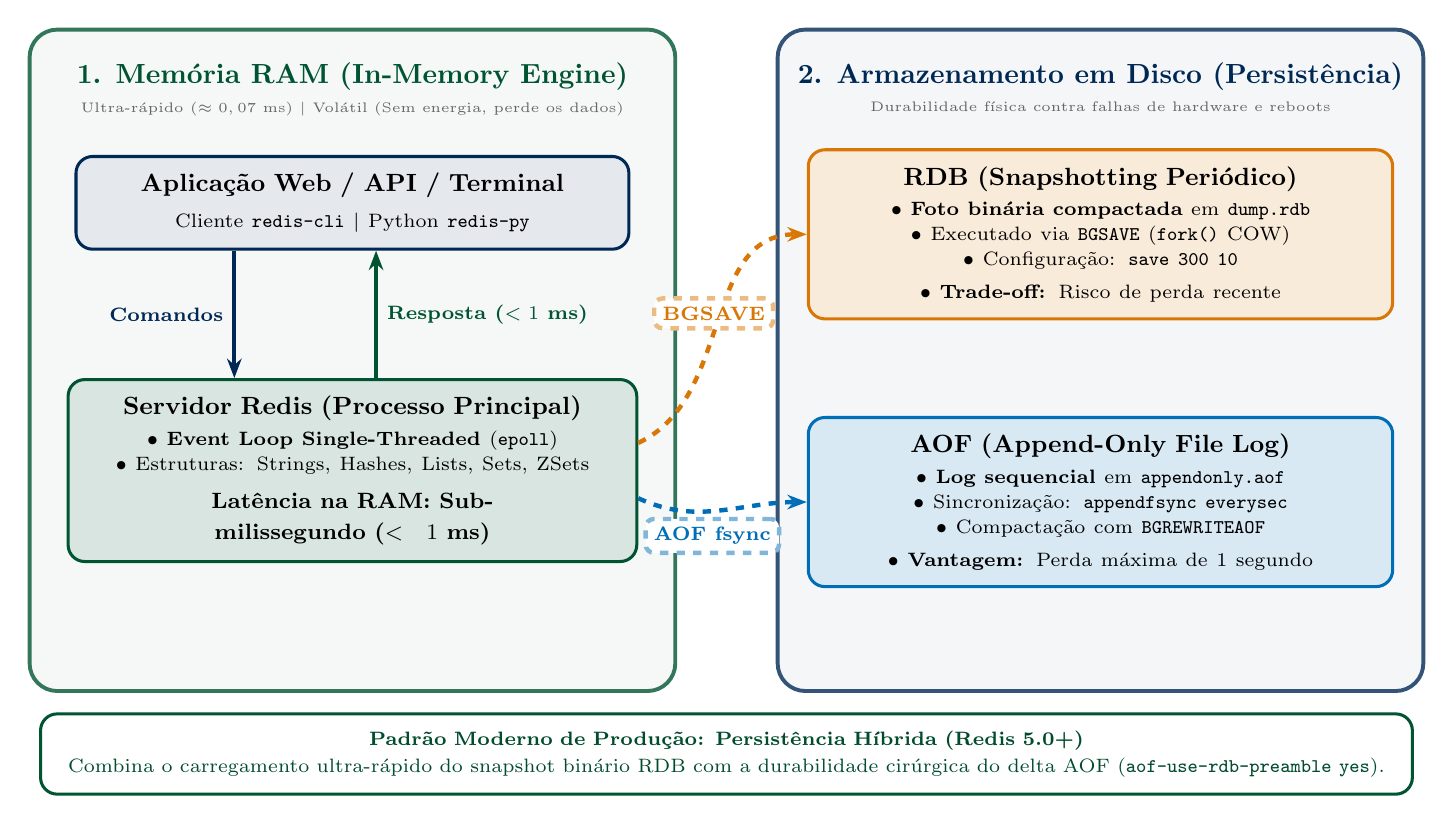
\begin{tikzpicture}[
    font=\sffamily,
    box/.style={draw=BorderGray, rounded corners=6pt, fill=white, line width=1.1pt, align=center, inner sep=6pt},
    arrow/.style={-{Stealth[length=7pt]}, line width=1.4pt}
]

  % =========================================================================
  % PAINEL ESQUERDO: MEMÓRIA RAM (MOTOR PRINCIPAL IN-MEMORY)
  % =========================================================================
  \node[draw=ScoutGreen!80, rounded corners=10pt, fill=ScoutGreen!4, line width=1.4pt, minimum width=8.2cm, minimum height=8.4cm] (p_ram) at (4.1, 3.2) {};
  
  \node[font=\bfseries\normalsize, text=ScoutGreen, anchor=north] at (4.1, 7.1) {1. Memória RAM (In-Memory Engine)};
  \node[font=\tiny, text=gray!80!black, anchor=north] at (4.1, 6.6) {Ultra-rápido ($\approx 0,07$ ms) $\mid$ Volátil (Sem energia, perde os dados)};

  % Aplicação / API
  \node[box, fill=ScoutNavy!10, draw=ScoutNavy, text width=6.6cm, font=\small] (app) at (4.1, 5.2) {
    \textbf{Aplicação Web / API / Terminal}\\[2pt]
    \scriptsize Cliente \texttt{redis-cli} $\mid$ Python \texttt{redis-py}
  };

  % Servidor Redis (RAM)
  \node[box, fill=ScoutGreen!15, draw=ScoutGreen, text width=6.8cm, font=\small] (redis_core) at (4.1, 1.8) {
    \textbf{Servidor Redis (Processo Principal)}\\[3pt]
    \scriptsize $\bullet$ \textbf{Event Loop Single-Threaded} (\texttt{epoll})\\[1pt]
    \scriptsize $\bullet$ Estruturas: Strings, Hashes, Lists, Sets, ZSets\\[3pt]
    \footnotesize \textbf{Latência na RAM: Sub-milissegundo ($< 1$ ms)}
  };

  % Setas verticais entre App e Redis
  \draw[arrow, color=ScoutNavy] ([xshift=-1.5cm]app.south) -- node[left, font=\scriptsize\bfseries, text=ScoutNavy] {Comandos} ([xshift=-1.5cm]redis_core.north);
  \draw[arrow, color=ScoutGreen] ([xshift=0.3cm]redis_core.north) -- node[right, font=\scriptsize\bfseries, text=ScoutGreen] {Resposta ($< 1$ ms)} ([xshift=0.3cm]app.south);

  % =========================================================================
  % PAINEL DIREITO: DISCO (PERSISTÊNCIA NÃO-VOLÁTIL)
  % =========================================================================
  \node[draw=ScoutNavy!80, rounded corners=10pt, fill=ScoutNavy!4, line width=1.4pt, minimum width=8.2cm, minimum height=8.4cm] (p_disk) at (13.6, 3.2) {};
  
  \node[font=\bfseries\normalsize, text=ScoutNavy, anchor=north] at (13.6, 7.1) {2. Armazenamento em Disco (Persistência)};
  \node[font=\tiny, text=gray!80!black, anchor=north] at (13.6, 6.6) {Durabilidade física contra falhas de hardware e reboots};

  % Bloco RDB (Superior direito)
  \node[box, fill=ScoutAmber!15, draw=ScoutAmber, text width=7.0cm, font=\small] (rdb_box) at (13.6, 4.8) {
    \textbf{RDB (Snapshotting Periódico)}\\[3pt]
    \scriptsize $\bullet$ \textbf{Foto binária compactada} em \texttt{dump.rdb}\\[1pt]
    \scriptsize $\bullet$ Executado via \textbf{\texttt{BGSAVE}} (\texttt{fork()} COW)\\[1pt]
    \scriptsize $\bullet$ Configuração: \texttt{save 300 10}\\[1pt]
    \scriptsize $\bullet$ \textbf{Trade-off:} Risco de perda recente
  };

  % Bloco AOF (Inferior direito)
  \node[box, fill=ScoutBlue!15, draw=ScoutBlue, text width=7.0cm, font=\small] (aof_box) at (13.6, 1.4) {
    \textbf{AOF (Append-Only File Log)}\\[3pt]
    \scriptsize $\bullet$ \textbf{Log sequencial} em \texttt{appendonly.aof}\\[1pt]
    \scriptsize $\bullet$ Sincronização: \textbf{\texttt{appendfsync everysec}}\\[1pt]
    \scriptsize $\bullet$ Compactação com \textbf{\texttt{BGREWRITEAOF}}\\[1pt]
    \scriptsize $\bullet$ \textbf{Vantagem:} Perda máxima de 1 segundo
  };

  % Setas de conexão da RAM para o Disco (Canal central amplo e sem sobreposição)
  \draw[arrow, color=ScoutAmber, dashed, line width=1.6pt] ([yshift=10pt]redis_core.east) to[out=25, in=180]
    node[pos=0.45, above=2pt, font=\scriptsize\bfseries, text=ScoutAmber, fill=white, inner sep=3pt, rounded corners=3pt, draw=ScoutAmber!50] {BGSAVE} (rdb_box.west);

  \draw[arrow, color=ScoutBlue, dashed, line width=1.6pt] ([yshift=-10pt]redis_core.east) to[out=-25, in=180]
    node[pos=0.45, below=2pt, font=\scriptsize\bfseries, text=ScoutBlue, fill=white, inner sep=3pt, rounded corners=3pt, draw=ScoutBlue!50] {AOF fsync} (aof_box.west);

  % =========================================================================
  % FAIXA INFERIOR: PERSISTÊNCIA HÍBRIDA
  % =========================================================================
  \node[draw=ScoutGreen, fill=white, rounded corners=6pt, font=\scriptsize, align=center, text=ScoutGreen!90!black, line width=1.1pt, text width=17.0cm, inner sep=6pt] at (8.85, -1.8) {
    \textbf{Padrão Moderno de Produção: Persistência Híbrida (Redis 5.0+)}\\[2pt]
    Combina o carregamento ultra-rápido do snapshot binário RDB com a durabilidade cirúrgica do delta AOF (\texttt{aof-use-rdb-preamble yes}).
  };

\end{tikzpicture}
\end{document}
